\input ../preamble

\begin{document}

{\Huge

  \centerline{\bf TTIC 31230, Fundamentals of Deep Learning}
  \bigskip
  \centerline{David McAllester, Winter 2018}

  \vfill
  \centerline{\bf Information Theory} 
  \vfill
\vfill
\vfill

\slide{Logistic Regression as a Major Advance}


$$\Phi^* = \argmin_\Phi \;E_{(x,y) \sim \mathrm{Train}} \;(y-f_\Phi(x))^2$$

\vfill
Switched to

\vfill
\begin{eqnarray*}
  Q_\Phi(y|x) & = & \softmax_{\hat{y}}\;f_\Phi(\hat{y}|x) \\
  \\
  \Phi^* & = & \argmin_\Phi\;E_{(x,y) \sim \mathrm{Train}}\;\; - \log\;Q_\Phi(y|x)
\end{eqnarray*}


\slide{Binary Classification}

We have a population distribution over $(x,y)$ with $y \in \{-1,1\}$.

\vfill
We compute a single number $f_\Phi(x)$ where

\vfill
for $f_\Phi(x) \geq 0$ predict $y = 1$

\vfill
for $f_\Phi(x) < 0$ predict $y = -1$

\slide{Softmax for Binary Classification}

\begin{eqnarray*}
  Q_\Phi(y|x) & = & \frac{1}{Z} \;e^{yf(x)} \\
  \\
  & = & \frac{e^{yf(x)}}{e^{yf(x)} + e^{-yf(x)}} \\
  \\
  \\
  & = & \frac{1}{1 + e^{-2yf(x)}} \\
  \\
  \\
    & = & {\color{red} \frac{1}{1 + e^{-m(y)}}} \;\;\;\;\;\;m(y|x) = 2yf(x)\;\mbox{is the margin}
\end{eqnarray*}

\slide{Logistic Regression for Binary Classification}

\begin{eqnarray*}
  \Phi^* & = & \argmin_\Phi\;E_{(x,y) \sim \mathrm{Train}}\;\ln 1/Q_\Phi(y|x) \\
  \\
  & = & \argmin_\Phi\;E_{(x,y) \sim \mathrm{Train}}\;{\color{red} \ln \left(1 + e^{-m(y|x)}\right)} \\
  \\
  \ln \left(1 + e^{-m(y|x)}\right) & \approx & 0 \;\;\;\mbox{for $m(y|x) >> 1$} \\
  \\
  \ln \left(1 + e^{-m(y|x)}\right) & \approx & -m(y|x) \;\;\;\mbox{for $m(y|x) << -1$} \\
\end{eqnarray*}

\slide{Log Loss vs. Hinge Loss}
Log loss:
\begin{eqnarray*}
  \Phi^* & = & \argmin_\Phi\;E_{(x,y) \sim \mathrm{Train}}\;- \ln Q_\Phi(y|x) \\
  \\
  & = & \argmin_\Phi\;E_{(x,y) \sim \mathrm{Train}}\;\ln \left(1 + e^{-m(y|x)}\right)\;\;\;\;\;\mbox{binary case}
\end{eqnarray*}

\vfill
Hinge Loss:
\begin{eqnarray*}
  \Phi^* & = & \argmin_\Phi\;E_{(x,y) \sim \mathrm{Train}}\;\max(0,1-m(y|x)) \\
  \\
  m(y|x) & = & \min_{\hat{y} \not = y} \;f(y|x) - f(\hat{y}|x)
\end{eqnarray*}

\slide{Log Loss vs. Hinge Loss}

We will show that log loss is a consistent probability estimator.

\vfill
For log loss, and for infinite training data, $Q^*(y|x)$ is the true population conditional probability.

\vfill
Hinge loss is a consistent classifier but not a consistent probability estimator.
\begin{eqnarray*}
  f^*(y^*|x) & = & 1 \\
  f^*(\hat{y}|x) & = & 0 \;\;\;\mbox{for $\hat{y} \not = y^*$}
\end{eqnarray*}


\slide{Entropy}

Consider a probability distribution $\mathrm{Pop}$ on a finite set $S$.

\vfill
Consider a code $C$ assigning a bit string code word $C(y_1,\ldots,y_B)$ to each possible batch of $B$ elements with $y_i \sim \mathrm{Pop}$.

\vfill
Source coding theorem: As $B \rightarrow \infty$ the optimal coding uses exactly
$${\color{red} H(\mathrm{Pop}) = E_{y\sim \mathrm{Pop}}\; - \log_2 \mathrm{Pop}(y)}$$
bits per batch element.

\slide{Prefix Free Codes}

Let $S$ be a finite set.

\vfill
Let $C$ be assignment of a bit string $C(y)$ to each $y \in S$.

\vfill
$C$ is called {\em prefix-free} if for $x \not = y$ we have that $C(x)$ is not a prefix of $C(y)$.

\vfill
A concatenation of sequence of prefix-free code words can be uniquely segmented (parsed) back into a sequence of code words.

\slide{Prefix-Free Codes as Trees and as Probabilities}

A prefix-free code defines a binary branching tree --- branch on the first code bit, then the second, and so on.

\vfill
The leaves of this tree are labeled with the elements of $S$.

\vfill
The code defines a probability distribution on $S$ by randomly selecting branches.

\vfill
We have $Q_C(y) = 2^{-|C(y)|}$.

\slide{The Source Coding Theorem}

(1) There exists a prefix-free code $C$ such that
$$|C(y)| <= (- \log_2 \mathrm{Pop}(y)) + 1$$
and hence
$$E_{y\sim \mathrm{Pop}} |C(y)| \leq H(\mathrm{Pop}) +1$$

\vfill
(2) For any prefix-free code $C$

$$E_{y \sim \mathrm{Pop}}\;|C(y)| \geq H(\mathrm{Pop})$$

\slide{Code Construction}

\vfill
We construct a code by iterating over $y \in S$ in order of decreasing probability (most likely first).

\vfill
For each $y$ select a code word $C(y)$ (a tree leaf) with length (depth)

\vfill
$$|C(y)| = \lceil - \log_2 \mathrm{Pop}(y)\rceil$$

\vfill
and where $C(y)$ is not an extension of (under) any previously selected code word.

\slide{Code Existence Proof}

At any point before coding all elements of $S$ we have
$$\sum_{y \in \mathrm{Defined}} 2^{-|C(y)|} \leq \sum_{y \in \mathrm{Defined}} \mathrm{Pop}(y) < 1$$

\vfill
Therefore there exists an infinite descent into the tree that misses all previous code words.

\vfill
Hence there exists a code word $C(x)$ not under any previous code word with
$|C(x)| = \lceil - \log_2 \mathrm{Pop}(y)\rceil$.

\vfill
Furthermore $C(x)$ is at least as long as all previous code words and hence $C(x)$ is not a prefix of any previously selected code word.

\slide{Huffman Coding}

Maintain a list of trees $T_1,\;\dots,\;T_N$.

\vfill
Inititally each tree is just one root node labeled with an element of $S$.

\vfill
Each tree $T_i$ has a weight equal to the sum of the probabilities of the nodes on the leaves of that tree.

\vfill
Repeatedly merge the two trees of lowest weight into a single tree until all trees are merged.

\slide{Optimality of Huffman Coding}

{\bf Theorem}: The Huffman code $T$ for $\mathrm{Pop}$ is optimal --- for any other tree $T'$ we have $d(T;\mathrm{Pop}) \leq d(T';\mathrm{Pop})$.

\vfill
{\bf Proof}: The algorithm maintains the invariant that there exists an optimal tree including
all the subtrees on the list.

\vfill
To prove that a merge operation maintains this invariant we consider any tree containing the given subtrees.

\vfill
Consider the two subtrees $T_i$ and $T_j$ of minimal weight.  Without loss of generality we can assume that $T_i$ is at least as deep as $T_j$.

\vfill
Swapping the sibling of $T_i$ for $T_j$ brings $T_i$ and $T_j$ together and can only improve the average depth.

\slide{Optimality of Huffman Coding}

Why the swap operation cannot increase entropy. ...

\slide{Back to Log Loss}

Log loss has both a conditional and an unconditional version.

\vfill
\begin{eqnarray*}
  \Phi^* & = & \argmin_\Phi \;\;E_{(x,y) \sim \mathrm{Pop}}  -\log Q_\Phi(y|x) \\
  \\
  \\
  \Phi^* & = & \argmin_\Phi \;\;E_{y \sim \mathrm{Pop}}  -\log Q_\Phi(y)
\end{eqnarray*}

Conditional test loss can often be made small (MNIST, speech recognition) but can also be inherently large (image colorization).

\vfill
Unconditional log loss is typically inherently large (language modeling).

\vfill
\slide{Log Loss is Cross Entropy}


\begin{eqnarray*}
  H(\mathrm{Pop}) & \doteq & E_{y \sim \mathrm{Pop}}\;- \log \mathrm{Pop}(y) \\
  \\
  H(\mathrm{Pop},Q) & \doteq & E_{y \sim \mathrm{Pop}}\; -\log\; Q(y) \\
  \\
  \\
  E_{y \sim \mathrm{Pop}} -\log Q_\Phi(y)  & = & H(\mathrm{Pop},Q_\Phi) \\
  \\
  \\
  E_{(x,y) \sim \mathrm{Pop}} -\log Q_\Phi(y|x)  & = & E_{x \sim \mathrm{Pop}} \; H(\mathrm{Pop}(y|x),Q_\Phi(y|x)) \\
\end{eqnarray*}


\slide{KL Divergence}

\begin{eqnarray*}
  KL(\mathrm{Pop},Q) & \doteq & E_{y \sim \mathrm{Pop}} \;\log_2 \frac{\mathrm{Pop}(y)}{Q(y)} \\
  \\
  & = & E_{y \sim \mathrm{Pop}} \;\log \mathrm{Pop}(y) - \log Q(y) \\
  \\
  & = & \left(E_{y \sim \mathrm{Pop}} \; - \log Q(y)\right) - \left(E_{y \sim \mathrm{Pop}} \; - \log \mathrm{Pop}(y)\right) \\
  \\
  & = & H(\mathrm{Pop},Q) - H(P)
\end{eqnarray*}

\slide{Jensen's Inequality}

\centerline{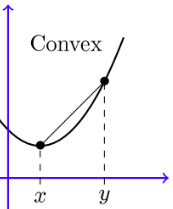
\includegraphics[height = 3.0in]{../images/Jensen}}

\vfill
For $f$ convex (upward curving) we have

\vfill
$$E[f(x)] \geq f(E[x])$$

\slide{KL Divergence}

\begin{eqnarray*}
  KL(P,Q) & = & \expectsub{y \sim P}{- \log \frac{Q(y)}{P(y)}} \\
  \\
  & \geq & - \log \expectsub{x\sim P}{\frac{Q(y)}{P(y)}} \\
  \\
  & = & - \log \sum_y\; P(y) \frac{Q(y)}{P(y)}  \\
  \\
  & = & - \log \sum_y Q(y) \\
  \\
  & = & 0
\end{eqnarray*}

\slide{Fundamentals}

\begin{eqnarray*}
  KL(\mathrm{Pop},Q) & \geq & 0 \\
  \\
  H(\mathrm{Pop},Q) & = & H(\mathrm{Pop}) + KL(\mathrm{Pop},Q) \\
  \\
  & \geq & H(\mathrm{Pop}) \\
  \\
  \argmin_Q H(\mathrm{Pop},Q) & = & \mathrm{Pop} \\
  \\
  \argmin_{Q(y|x)}\;E_{x \sim \mathrm{Pop}}\; H(\mathrm{Pop(y|x)}, Q(y|x)) & = & \mathrm{Pop}(y|x) \\
\end{eqnarray*}
    
\slide{Asymmetry of Cross Entropy}
Consider 


$$\Phi^* = \argmin_\Phi \;H(P,Q_\Phi)\;\;\;\;\;(1)$$

\vfill
$$\Phi^* = \argmin_\Phi \;H(Q_\Phi,P)\;\;\;\;\;(2)$$

\vfill
For (1) $Q_\Phi$ must cover all of the support of $P$.

\vfill
For (2) $Q_\Phi$ concentrates all mass on the point maximizing $P$.

    
\slide{Asymmetry of KL Divergence}
Consider 


\begin{eqnarray*}
  \Phi^* & = & \argmin_\Phi \;KL(P,Q_\Phi) \\
  & = & \argmin_\Phi\; H(P,Q_\Phi)\;\;\;\;\;\;\;\;\;\;\;\;\;\;\;\;\;\;(1) \\
  \\
  \Phi^* & = & \argmin_\Phi \;KL(Q_\Phi,P) \\
  & = & \argmin_\Phi H(Q_\Phi,P) - H(Q_\Phi)\;\;\;(2)
  \end{eqnarray*}

\vfill
If $Q_\Phi$ is not universally expressive we have that (1) still forces $Q_\Phi$ to cover all of $P$ (or else the KL divergence is infinite)
while (2) allows $Q_\Phi$ to be restricted to a single mode of $P$ (a common outcome).

\slideplain{Unsupervised Learning}

Unsupervised learning is sometimes equated with unconditional log loss (density estimation).

\vfill
\begin{eqnarray*}
  \Phi^* & = & \argmin_\Phi \;\;E_{y \sim \mathrm{Pop}}  -\log Q_\Phi(y)
\end{eqnarray*}

\slide{Unsupervised Learning}

\centerline{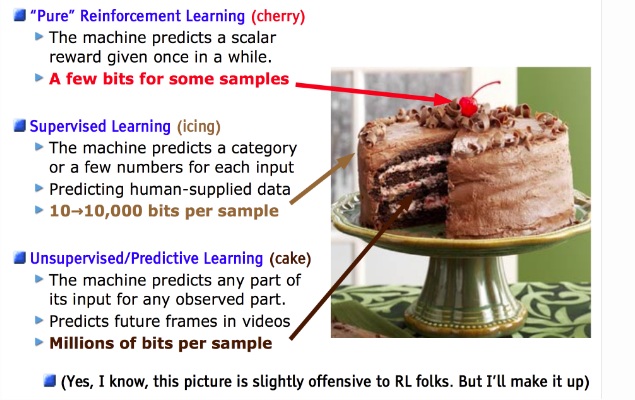
\includegraphics[width = 8in]{../images/cake}}


\slide{Unsupervised Learning}

By ``unsupervised learning'' we will mean learning from {\bf massively available} data.  This is not a mathematical definition.

\vfill
{\bf Massive}: images, audio, text, video, click-through data.

\vfill
{\bf Less Massive}: car control data, stereo image pairs, closed captioned video, captioned images.

\vfill
{\bf Big}: Manually annotated images or audio.

\vfill
{\bf Small}: manually annotated text --- parse trees, named entities, semantic roles, coreference, entailment.

\vfill
{\bf Smallest:} Manually annotated text in an obscure language.

\slide{Colorization}

$$\Phi^* = \argmin_\Phi \expectsub{(x,y) \sim \mathrm{Pop}}{-\log Q_\Phi(y|x)}$$

\vfill
\centerline{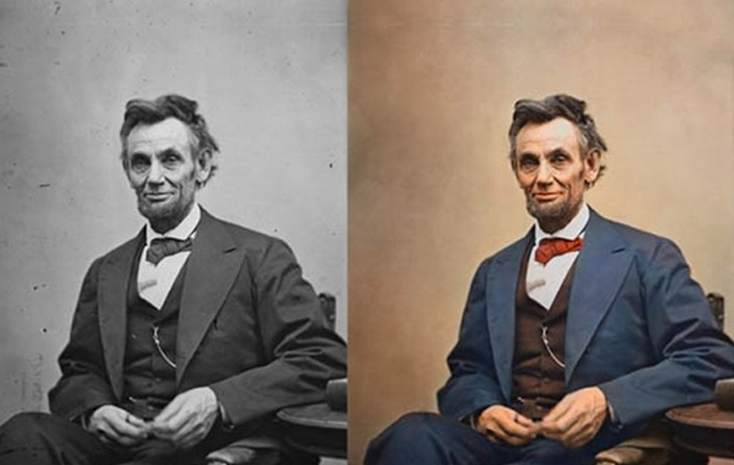
\includegraphics[height=2in]{../images/Colorization}}

\vfill
We have massive data for colorization.

\vfill
But any colorization is inevitably a guess.

\slide{Differential Entropy}

Consider a continuous density $p(x)$.  For example

\vfill
$$p(x) = \frac{1}{\sqrt{2\pi}\; \sigma}\; e^{\frac{-x^2}{2\sigma^2}}$$

\vfill
Differential entropy is often defined as

\vfill
$$H(p) \doteq \int \left(\ln \frac{1}{p(x)}\right) p(x) dx$$

\slide{Finite Differential Entropy is Not Meaningful}

\begin{eqnarray*}
  H({\cal N}(0,\sigma)) & = &  + \int \left( \ln(\sqrt{2\pi} \sigma) + \frac{x^2}{2\sigma^2}\right) p(x) dx \\
  \\
  & = & \ln(\sigma) + \ln(\sqrt{2\pi}) + \frac{1}{2}
\end{eqnarray*}

\vfill
But if we take $y \doteq x/2$ we get $H(y) = H(x) - \ln 2$.

\vfill
Also for $\sigma << 1$, we get $H(p) < 0$

\vfill
Hence differential entropy then depends on the choice of units --- a distributions on lengths will have a different entropy
when measuring in inches than when measuring in feet.

\slide{Differential Entropy is Always Infinite}

Consider quantizing the the real numbers into bins.

\vfill
A continuous probability densisty $p$ assigns a probability $p(B)$ to each bin.

\vfill
As the bin size decreases toward zero the entropy of the bin distribution increases toward $\infty$.

\vfill
A meaningful convention is that $H(p) = +\infty$ for any continuous density $p$.

\slide{Differential KL-divergence is Meaningful}

$$KL(p,q) = \int \left( \ln \frac{p(x)}{q(x)}\right) p(x) dx$$

\vfill
This integral can be computed by dividing the real numbers into bins and computing the $KL$ divergence between the distributions on bins.

\vfill
The KL divergence between the bin distribution typically approaches a finite limit as the bin size goes to zero.

\slide{KL-Divergence can also be Infinite}

$$KL(p,q) = E_{x \sim p}\; \log\frac{p(x)}{q(x)}$$
\vfill
In either the discrete or continuous case, if a set is assigned nonzero probability by $p$ but zero probability by $q$ then $KL(p,q) = +\infty$.

\vfill
If every set assigned nonzero probability by $p$ is also assigned nonzero probability by $q$ then we say that $p$ is absolutely continuous with respect to $q$.

\slide{Random Variables}

We consider variables where a single draw form the population determines a value for each variable.

\vfill
This is the formal definition of a ``random variable''.

\vfill
Each random variable has a probability distribution defined by the distribution on the population.

\vfill
We write $H(x)$ for the entropy of the distribution on $x$.

\slide{Mutual Information}

For two random variables $x$ and $y$ there is a distribution on pairs $(x,y)$ determined by the population distribution.

\vfill
Mutual information concerns the relationship between the distribution on $(x,y)$ and the marginal distributions on $x$ and $y$.

\vfill
For the discrete case we can write.

\vfill
\begin{eqnarray*}
  I(x,y) & \doteq & H(x) + H(y) - H(x,y)
\end{eqnarray*}

\vfill
This can be viewed as a quantity of non-independence --- independent variables have zero mutual information.

\slide{Conditional Entropy}

For the discrete case conditional entropy $H(y|x)$ is defined by

\begin{eqnarray*}
  H(y|x) & \doteq & \sum_x \mathrm{Pop}(x) \sum_y \mathrm{Pop}(y|x) - \log \mathrm{Pop}(y|x) \\
  \\
  & = & E_{x\sim \mathrm{Pop}}\;E_{y \sim \mathrm{Pop}|x}\;- \log \mathrm{Pop}(y|x) \\
  \\
  & = & E_{x\sim \mathrm{Pop}}\;H(\mathrm{Pop}(y|x))
\end{eqnarray*}

\slide{More Identities}
\vfill
For the discrete case we have.

\vfill
\begin{eqnarray*}
  I(x,y) & = & H(x) - H(x|y) \\
  \\
  & = & H(y) - H(y|x) \\
  \\
  & = & KL(\mathrm{Pop}(x,y),\mathrm{Pop}(x)\times\mathrm{Pop}(y))
\end{eqnarray*}

The last identity can be taken as a definition of $I(x,y)$ in the continuous case.

\slide{END}

}
\end{document}
